\chapter{Umsetzung \& Konzeption}
\label{chap:umsetzung}

	Während im \autoref{chap:projektablauf} sowohl die grundlegenden Ansätze der Projektorganisation, als auch ein essentielles Tool aufgeführt wurden, hat sich das \autoref{chap:SpecCustom} mit den im Customizing anfallenden Aufgaben befasst. In Folgenden soll ein Modell erstellt werden, welches die wichtigsten Aufgaben in einem Customizingprojekt in eine adäquate Reihenfolge setzt, sowie einen grob strukturierten Ablaufplan anhand eines \acs{PSP} erstellt. Dieser Plan soll zukünftig dabei helfen Aufgaben schneller und effizienter zu Identifizieren. Außerdem soll dieser als eine Art Checkliste eingesetzt werden können. 
	
\section*{Modell}

	Um ein Modell erzeugen zu können, müssen in erster Linie die Zusammenhänge zwischen unterschiedlichen Projekten hergestellt werden. Da diese Ausarbeitung sich mit dem Thema des Customizings befasst, werden nur diese berücksichtigt. Wie im \autoref{chap:SpecCustom} beschrieben, befasst sich diese Art von Projekten stets mit dem selben Set von Aufgaben. Daher kann davon ausgegangen werden, dass ein Zusammenhang bei dieser Art von Projekten besteht.
	Ist der Zusammenhang einmal klar, so muss die Strukturierung der Herangehensweise an das Projekt geklärt werden, da das Customizing zwar die Aufgabenstellungen sequenziell abarbeitet, jedoch wegen sich ändernden Anforderungen der Kunden eine iterative Vorgehensweise gegeben sein muss, sollte hier ein hybrides vorgehen angedacht werden. Somit kann es in einzelnen Phasen zu Iterationen kommen. Daher ist zu empfehlen sowohl zwischen sich wiederholenden Aufgaben als auch einmaligen zu unterscheiden. 
	
	Da ein \acs{PSP} objektorientiert, funktionsorientiert oder phasenorientiert aufgebaut werden kann, ist hier zudem eine Auswahl notwendig. Diese findet sich im Bereich des Customizings wegen einem verstärkten Bezug zu dem Projektmanagement im phasenorientierten Ansatz wieder. 
	Somit ist es empfehlenswert den \acs{PSP} nach den einzelnen Phasen des im \autoref{chap:projektablauf} beschriebenen Lebenszyklus zu gliedern. Vor einer Festlegung der Arbeitspakete sollte die Definition der Aufgaben erstellt werden. Die so erarbeiteten Aufgaben können anschließend zu Arbeitspaketen gegliedert werden. 
	Als Unterstützung dienen hierbei die definierten Customizing- Aufgaben im \autoref{sec:aufgabenCustomizing}. Für die Bewahrung einer stringenten Form wurde das \acs{AP} im \autoref{sec:arbeitspakete} beschrieben. Diese hilft dem Benutzer die wichtigsten Informationen zu erfassen, damit im späteren Vorgehen keine Lücken entstehen. Das von Känel zur Verfügung gestellte Layout (\autoref{img:arbeitspaket}) hilft dem Benutzer eine replizierbare Form herzustellen. Nachdem ein solches \acs{AP} entsteht, findet eine Zuordnung zum \acs{PSP} statt. Eine genaue Zeitliche Reihenfolge kann hier allerdings nicht ausgearbeitet werden, da sich die Aufgaben je nach Umfang des Projektes unterscheiden. Genauso wenig lassen sich Aufgaben detailliert darstellen, da sowohl Dauer als auch Kosten von unterschiedlichen Faktoren abhängen. Daher sollte dieses Modell lediglich als Leitfaden dienen an dem sich ein Projektleiter orientieren kann. Die \autoref{img:PSP1} zeigt einen Entwurf, der sowohl die unterschiedlichen Phasen des Projektmanagements abdeckt, als auch dem Zeitlichen Ablauf zugeordnete Beispiel-Aufgaben beinhaltet.   
	
	\begin{figure}[h]
		\centering
		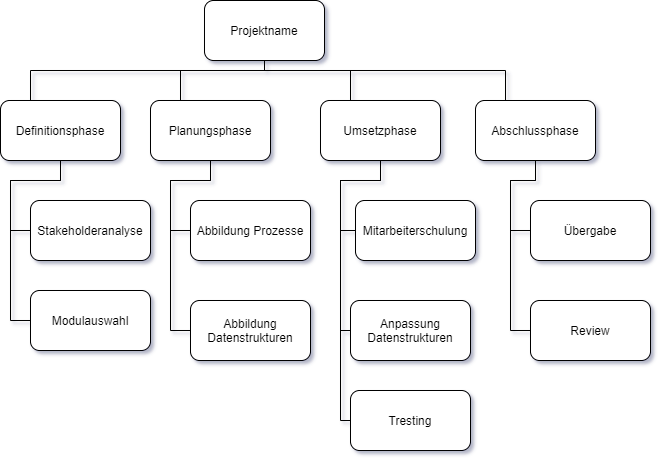
\includegraphics[width=15cm]{img/psp01.png}
		\caption{\ac{PSP}}
		\label{img:PSP1}
	\end{figure}
	
	
	
	
	